\documentclass[11pt]{article}

\usepackage{graphicx}
\usepackage[sorting=none]{biblatex}
\usepackage[margin=0.75in]{geometry}
\usepackage[colorlinks=true]{hyperref}
\usepackage{amsmath}
\usepackage{amssymb}
\usepackage[format=plain, labelfont=it, font=footnotesize, labelsep=period]{caption}
\usepackage{caption}
\usepackage{subcaption}
\usepackage{multicol}
\usepackage{wrapfig}
\usepackage{float}
\usepackage{lipsum}
\usepackage{subfiles}

\addbibresource{references.bib}

\title{Pendulum Lab Report III}
\author{Kevin (Zerui) Wang}
\date{\today}


\begin{document}

\pagenumbering{gobble}
\maketitle

\newpage

\pagenumbering{arabic}

\begin{multicols}{2}
\section{Introduction}
The purpose of this lab report is to evaluate the accuracy of various theoretical models used to predict the behaviour of a simple pendulum. Experiments demonstrate that there exists a relationship between period and release angle, amplitude and time, period and length, and Q factor and length. The following section presents all the theoretical background that these relationships are built upon.

\section{Background} \label{Background}
A simple pendulum can be defined as a weight suspended via a flexible string, below a pivot point to which it swings back and forth freely along a plane that contains the pivot point. The length of the pendulum is defined as the distance from the pivot point to the weight's center of mass. The following equation is used to describe a simple pendulum released from an angle $\theta$, provided that the mass of the string is negligible compared to the mass of the weight \cite{the-simple-pendulum}:
\begin{equation} \label{eq:l-over-g}
    T = 2\pi \sqrt{\frac{L}{g}}
\end{equation}
where:
{
\setlength{\abovedisplayskip}{2.5pt}
\begin{flalign*}
    \qquad L &= \text{pendulum length in cm} & \\ % \\[-3pt] for paragraphs
    % \qqquad &\phantom{{}={}} \text{ayo continuation br}\\
    \qquad g &= \text{acceleration due to gravity in m/s$^2$} & \\
    \qquad T &= \text{pendulum period in s} &
\end{flalign*}
}

More realistically, the behavior of an ideal pendulum assuming no energy loss due to friction can be modelled with a second order differential equation of $\theta$ with respect to $t$:
\begin{equation} \label{eq:diffeq-pendulum}
    \frac{d^2\theta}{dt^2} + \frac{g}{L}\sin{\theta} = 0
\end{equation}
where the solution $\theta(t)$ cannot be easily represented in terms of elementary functions \cite{no-elementary-fns}. Accordingly, the derived formula for $T(\theta)$ from Equation \ref{eq:diffeq-pendulum} is best described as an infinite series \cite{no-elementary-fns-2}:
\begin{align} \label{eq:power-series-derived}
\begin{split}
    T(\theta) &= 2\pi\sqrt{\frac{L}{g}} \left(1 + \frac{1}{4}\sin^2\frac{\theta}{2} \right. + \\
    &\phantom{{}=}\left. \frac{9}{64}\sin^4\frac{\theta}{2} + \frac{225}{2304}\sin^6\frac{\theta}{2} + \ldots \right)
\end{split}
\end{align}


It is observed that Equation \ref{eq:power-series-derived} equals Equation \ref{eq:l-over-g} when $\theta$ is extremely small. This is known as the small angle approximation of a pendulum and it holds (implying simple harmonic motion also holds) for \cite{the-simple-pendulum}:
\begin{equation} \label{eq:small-angle-approx}
    |\theta| \lesssim 20^{\circ}
\end{equation}

Additionally, all previous models demonstrate that pendulum period does not depends on mass of the weight.

Another way to realistically model a pendulum is to incorporate dampening from frictional forces given by the following equation \cite{damped-oscillations}:
\begin{equation} \label{eq:damped-harmonic-oscillator}
    \theta(t) = \theta_0 e^{-{t/\tau}} \cos\left(2\pi\frac{t}{T} + \phi_0\right)
\end{equation}
where:
{
\setlength{\abovedisplayskip}{2.5pt}
\begin{flalign*}
    \qquad \theta_0 &= \text{initial release angle in rad} & \\ % \\[-3pt] for paragraphs
    % \qqquad &\phantom{{}={}} \text{ayo continuation br}\\
    \qquad \phi_0 &= \text{angular phase shift in rad} & \\
    \qquad \tau &= \text{decay constant governing damping} &
\end{flalign*}
}

It can be inferred from Equation \ref{eq:damped-harmonic-oscillator} that $T$ is constant for this model, implying the presence of small angle approximation. Additionally, removing the cosine term yields the amplitude-time graph:
\begin{equation} \label{eq:amplitude-function}
    A(t) = \theta_0 e^{-{t/\tau}}
\end{equation}

In order to quantify a pendulum's damping, its Q factor may be used. The Q factor measures how damped an oscillator is and is defined as follows \cite{pnp-physics}:
\begin{equation} \label{eq:q-factor-formula}
    Q = \pi\frac{\tau}{T}
\end{equation}

The Q factor is also defined by the amount of oscillations it takes for a pendulum's amplitude to decay to $e^{-\pi} \approx 4\%$ of its release angle (initial amplitude). Qualitatively, when the Q factor is large, the pendulum comes to rest slower. When the Q factor is small, the pendulum comes to rest quicker.

Lastly, a model which separates air resistance with string friction may also be included. That is, the frictional force at the pivot is assumed to be proportional to angular velocity in the simplest case \cite{duke-pendulum}. Given that $\frac{d\theta}{dt} = \omega = v/r$:
\begin{equation} \label{eq:propto v}
    F_p \propto v
\end{equation}
and air resistance is assumed to be proportional to the pendulum's cross sectional area and velocity squared \cite{airdrag}:
\begin{equation} \label{eq:propto v2}
    F_d \propto Av^2
\end{equation}

\section{Period and Release Angle} \label{sec 3 period and release angle}

\subsection{Experimental Setup} \label{sec 3.1 experimental setup}
The initial setup for the pendulum was made by first taping a protractor to the edge of a desk. The weight was hanged by tying a piece of cotton string around a stainless steel quick link that was aligned to match the $90^{\circ}$ mark on the protractor. Extra tape was also used to reinforce the pivot point, made to be collinear with the $0^{\circ}$ and $180^{\circ}$ markings. An image of the experimental setup is shown below:

\begin{figure}[H]
    \centering
    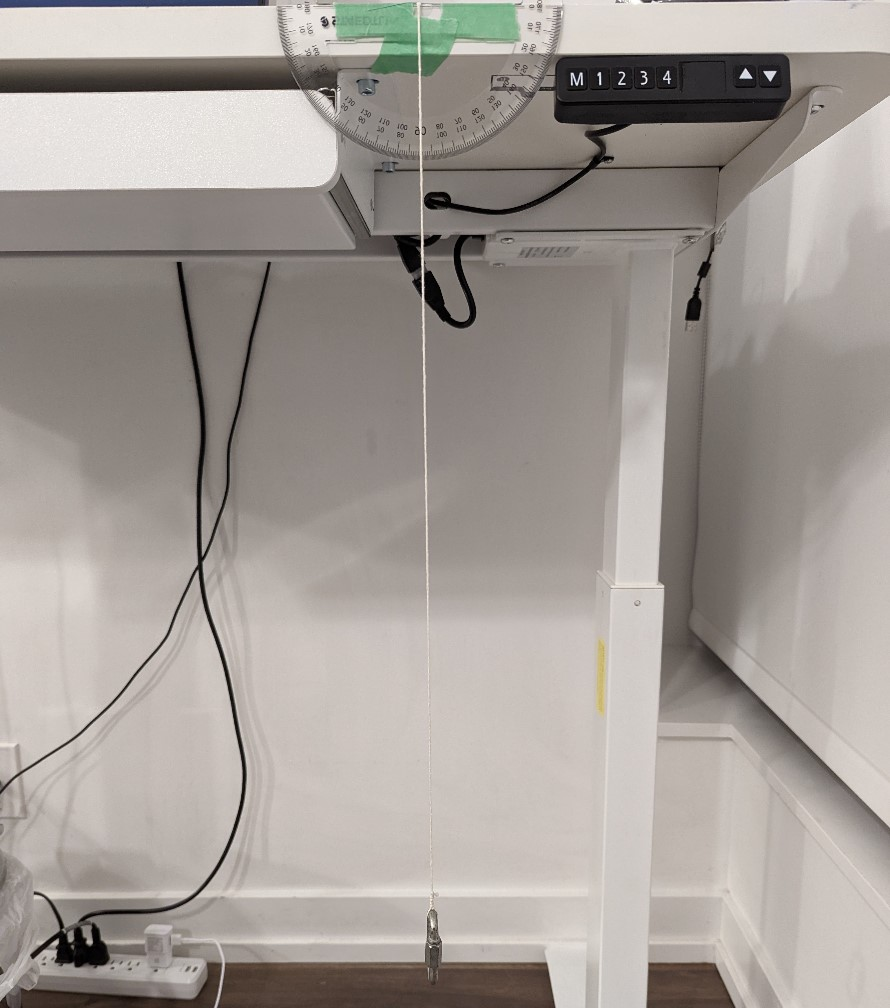
\includegraphics[width=\linewidth]{../figures/exp_setup1.jpg}
    \caption{\centering Picture of experimental setup for period vs. release angle data collection}
    \label{fig:figure 1}
\end{figure}


\subsection{Data} \label{sec 3.2 Data}
The data collected for the period vs. release angle graph is shown below:

\begin{figure}[H]
    \centering
    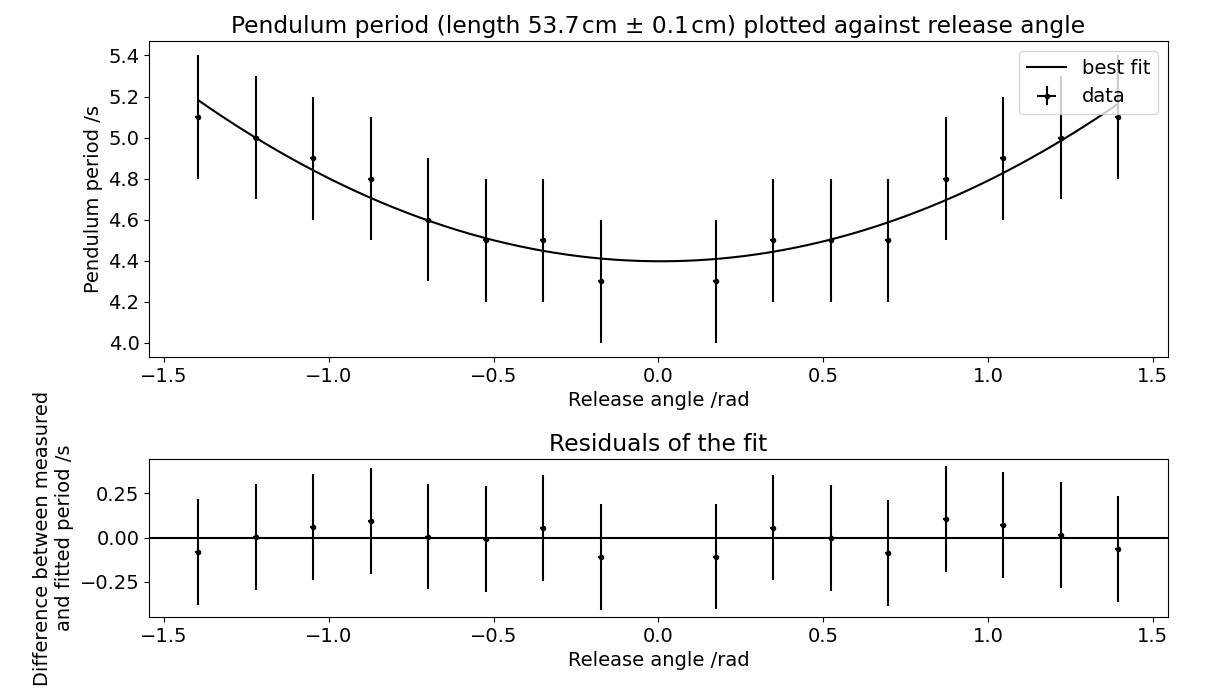
\includegraphics[width=\linewidth]{../figures/period_vs_release_angle.png}
    \caption{\centering Period plotted against release angle of the setup in Figure \ref{fig:figure 1}}
    \label{fig:figure 2}
\end{figure}

In total, the weight was released from 8 angles on both sides relative to the $90^{\circ}$ mark, starting from $10^\circ$ and taking increments of $10^\circ$ up to $80^\circ$. The uncertainty for each release angle was taken to $0.5^{\circ}$, the smallest increment on the protractor (converted to radians on graph). The period was measured by observing the pendulum for 3 swings and dividing the total time by 3, taking its maximum height as the reference point to reduce uncertainty in the weight's position (weight fastest at its lowest point). The period uncertainty was taken to be $0.25\,\text{s}$, the average human reaction time \cite{reaction-time}, since it is greater than the uncertainty of the stopwatch ($0.05\,\text{s}$) used.

All data collected were done without the need for tracking software.

\subsection{Analysis} \label{sec 3.3 analysis}
Qualitatively, the pendulum period stays relatively constant for small release angles. As release angle increases, the period deviates from the trend suggested by Equation \ref{eq:l-over-g}, taking on a symmetric, parabolic shape. Thus, a quadratic power series can be used to model this relationship, corresponding to the best-fit line from Figure \ref{fig:figure 2}:
\begin{equation} \label{eq:power series}
   T =  T_0(1 + B\theta_0 + C\theta_0^2)
\end{equation}
where:
{
\setlength{\abovedisplayskip}{2.5pt}
\begin{flalign*}
    \qquad \theta_0 &= \text{release angle in rad} & \\
    \qquad T_0 &= \text{smallest measured period}, (4.40\pm0.03)\,\text{s} & \\
    \qquad B &= -0.001\pm0.005 & \\
    \qquad C &= 0.091\pm0.007 &
\end{flalign*}
}

The uncertainties for unknown variables in the best-fit equation were calculated with a Python program.

By inspection, the calculated value of $T_0$ falls within the uncertainty range of the experimental value (period corresponding to release angle of $10^{\circ}$). The terms $B$ and $C$ are also significant because they describe the symmetry of parabola and how much it deviates from the trend described in Equation \ref{eq:l-over-g}. If $B \neq 0$, the parabola will not be centered at $\theta = 0$. Since the experimentally determined value of B is smaller than its uncertainty, it suffices to say that $B = 0$, implying symmetry in the graph. On the other hand, if $C = 0$, then the line of best-fit will have slope 0. However, this was determined experimentally to not be the case.

Given that the $r^2$ value is relatively close to 1, the residuals are both small and consistent, and the graph passes passes through all error bars, this fit would be a valid representation of the trend, implying that the pendulum period depends on release angle.

\section{Finding the Q Factor} \label{sec 4 Finding the Q Factor}

\subsection{Experimental Setup} \label{sec 4.1 experimental setup}
A single-stringed pendulum like the one presented in Subsection \ref{sec 3.1 experimental setup} tends to spin in an elliptical fashion when released, which violates the way a simple pendulum was defined in Section \ref{Background}. To correct for elliptical motion, a degree of freedom was removed from the pendulum by threading a string through the stainless steel quick link and fastening the threated string at 2 edge pivots to form the shape of a ``V''. This allows the pendulum to swing back and forth in the plane perpendicular to the ``V'' with the pivot point lying directly above the weight's center of mass. Lego pieces clamped down on the string to prevent it from slipping, and a protractor was taped directly above the weight, equidistant from the edge pivots. Extra caution was taken to ensure that the protractor's center, the edge pivots, and the camera lens were all aligned with each other. Shown below is a front view of the new setup:

\begin{figure}[H]
    \centering
    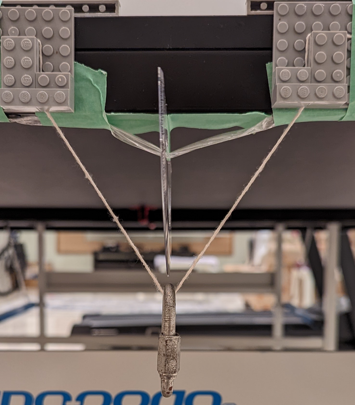
\includegraphics[width=\linewidth]{../figures/exp_setup3_front.png}
    \caption{\centering Improved version of the pendulum used to determine Q factor.}
    \label{fig:figure 3}
\end{figure}


\subsection{Data} \label{sec 4.2 data}
The Q factor can be determined by plotting
 data collected for the amplitude vs. time graph, as shown below:

\begin{figure}[H]
    \centering
    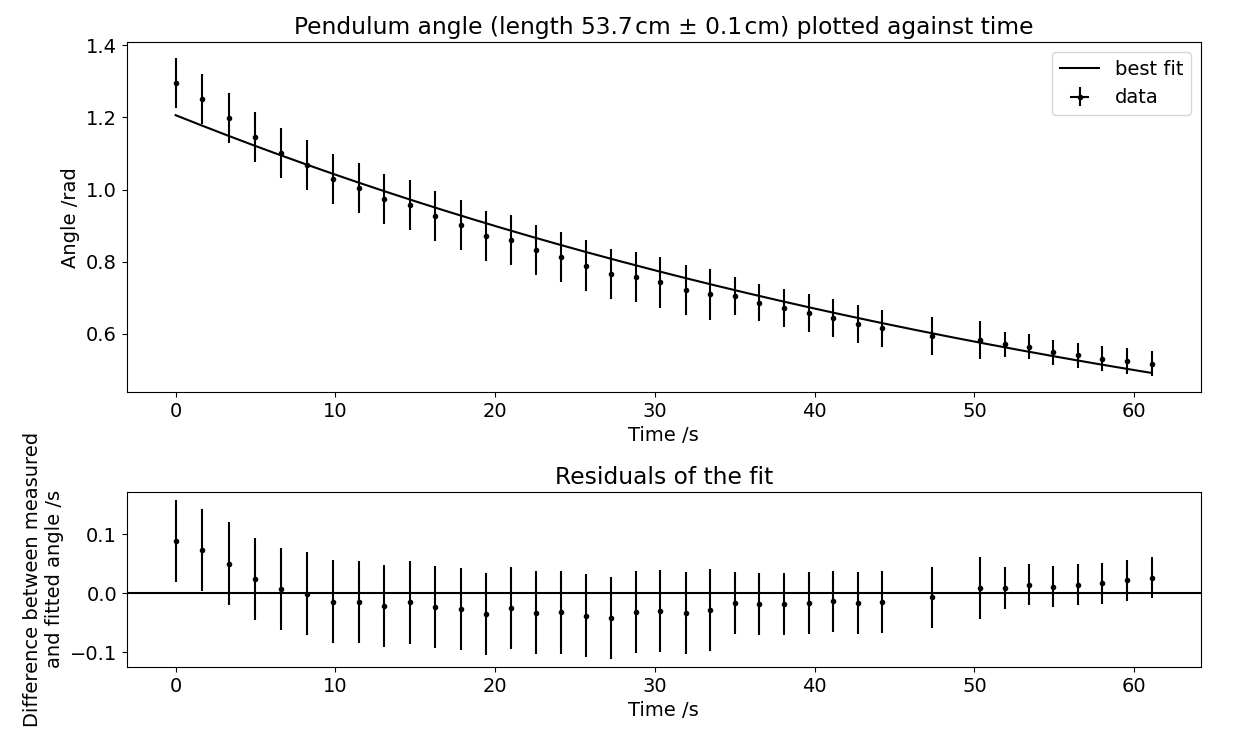
\includegraphics[width=\linewidth]{../figures/max_amplitude_vs_time.png}
    \caption{\centering Graph of maximum amplitude vs. time. This graph was initially generated inaccurately.}
    \label{fig:figure 4}
\end{figure}

The weight was released from an angle of approximately $20^\circ$ (within small angle approximation) to ensure that period stays constant as it is oscillating.  Initially, Figure \ref{fig:figure 4} was generated with a release angle of $60^\circ$, resulting the period to decrease with time due to frictional forces, producing an inaccurate Q factor.

To determine the amplitude at a given time, the full length of the video was divided into 15\,-\,20 equal intervals. For every interval, a few frames were moved forwards or backwards until the closest maximum amplitude was reached.

The value for each amplitude was measured in Tracker \cite{tracker} at the frame where the angle reached a local maximum specifically on the left side. When two strings appears in the frame due to camera skew, the angle was taken to be the midpoint of the region that the strings form. The uncertainty for angle would then equal half the absolute angle difference between the 2 strings. An image of angle calculation is shown below:

\begin{figure}[H]
    \centering
    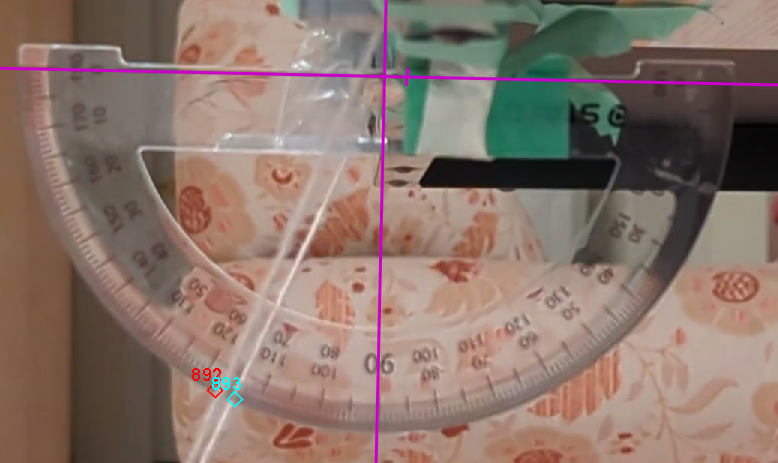
\includegraphics[width=\linewidth]{../figures/tracker.png}
    \caption{\centering Angle determination in Tracker. The red and blue points (coordinates relative to pink axis) highlight the region for angle measurement and uncertainty.}
    \label{fig:figure5}
\end{figure}

The uncertainty for time was taken to be 1/30 since the video was captured at 30 frames per second.

Although not plotted in the graph, the period was also needed for Q factor calculation. Using Tracker, period was measured by converting the number of frames taken for 5 swings into seconds, then dividing that value by 5. The uncertainty for period can then be reduced from 0.25\,s to 0.03\,s (same as time uncertainty) because Tracker allows the frame-by-frame playback and pausing of a video. For the specific setup described in this section, $T = (1.11 \pm 0.03)$\,s.

\subsection{Analysis} \label{sec 4.3 analysis}
The best-fit equation in Figure \ref{fig:figure 4} is modelled by Equation \ref{eq:amplitude-function} where:
{
\setlength{\abovedisplayskip}{2.5pt}
\begin{flalign*}
    \qquad \theta_0 &= (0.405 \pm 0.004)\,\text{rad} & \\
    \qquad \tau &= 170 \pm 2&
\end{flalign*}
}

Following a similar analysis to that of Subsection \ref{sec 3.3 analysis}, the calculated value for $\theta_0$ falls within the range of the measured value for $\theta_0$. Additionally, the very high $r^2$ value combined with small and consistent residuals suggests that damped harmonic motion (Equations \ref{eq:damped-harmonic-oscillator}, \ref{eq:amplitude-function}), provides a good fit for the data.

Given Equation \ref{eq:q-factor-formula} and a value for $T$ and $\tau$ with their uncertainties, the Q factor is calculated to be $480 \pm 14$, with its uncertainty taking on the higher percent uncertainty of $T$ and $\tau$.

Another way of determining the Q factor is by counting the number of oscillations as outlined in Section \ref{Background}.

Let $\theta_Q$ represent the amplitude at which the initial release angle decays to $e^{-\pi}\theta_0$. When $A(x) = \theta_Q$, $t_Q = 534$ seconds have elapsed, meaning $A(t_Q) = \theta_Q$. However, $\theta_Q$ carries an uncertainty of 0.009\,rad (Subsection \ref{sec 3.2 Data}), meaning $t_Q$ is bounded. When $A(x) = \theta_Q + 0.009$, $t = 465\,\text{s}$ and when $A(x) = \theta_Q - 0.009$, $t = 651\,\text{s}$. The uncertainty for $t_Q$ is taken to be the larger absolute difference of $t_Q$ from both bounds. Thus, the uncertainty for Q factor by counting oscillations is found by taking the larger percent uncertainty between $t_Q$ and $T$, resulting in $Q = 480 \pm 90$.

Although both methods yield the same value for Q factor, the counting method is not preferred due to its large uncertainty. The reason for this large uncertainty is attributed to the small rate of change of the exponential function $A(x)$ for large values of $t$.

\section{Period and Length} \label{sec 5 period and length}

\subsection{Experimental Setup} \label{sec 5.1 experimental setup}
The same pendulum and experimental setup in Subsection \ref{sec 4.1 experimental setup} was used to collect data for 9 different lengths ranging from $10\,$cm to $50\,$cm.

The angle formed by the ``V'' shape was kept at $60^\circ$ for all lengths due to ease of setup between trials, and also making sure that the dependent variable under investigation (period), will only depend on one independent variable (length).

The length of the pendulum was measured by taking the distance from the pivot point to the weight's center of mass, approximated to be at the center of the stainless steel quick link. Thus, length was taken to be the average of the distance from the pivot point to the top of the weight and the distance from the pivot point to the bottom of the weight.

For all lengths, angles were released from approximately $20^\circ$ for the same reasoning in Subsection \ref{sec 4.2 data}.

\subsection{Data} \label{sec 5.2 data}
The data collected for the period vs. length graph is shown below:

\begin{figure}[H]
    \centering
    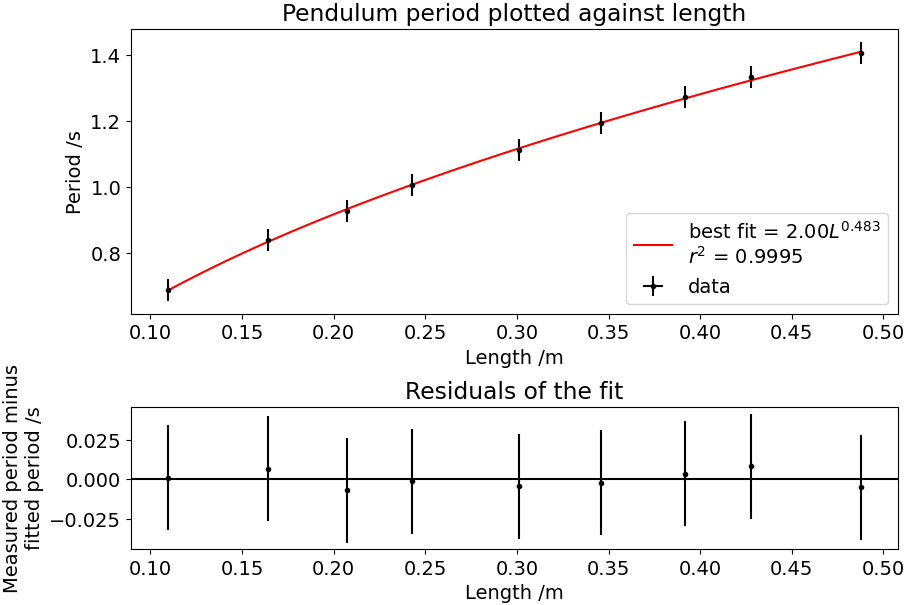
\includegraphics[width=\linewidth]{../figures/period_vs_length.png}
    \caption{\centering Graph of pendulum period plotted against pendulum length}
    \label{fig:figure 6}
\end{figure}

A tape measure was used to measure the pendulum's length. However, the uncertainty was taken to be double the smallest increment (0.05\,cm) of the tape measure since a double-ended measurement was used. The period measurement and its uncertainty was measured in the same was as Subsection \ref{sec 4.2 data}.

\subsection{Analysis} \label{sec 5.3 analysis}
The best-fit equation in Figure \ref{fig:figure 6} is modelled with a modified version of Equation \ref{eq:l-over-g} where:
{
\setlength{\abovedisplayskip}{2.5pt}
\begin{flalign*}
    \qquad A &\approx 2\pi/\sqrt{g} = 2.00 \pm 0.01 & \\ % \\[-3pt] for paragraphs
    % \qqquad &\phantom{{}={}} \text{ayo continuation br}\\
    \qquad n &= 0.483 \pm 0.004 &
\end{flalign*}
}

Given the 3\% difference from the fitted $n$ with the actual $n$, the very high $r^2$ value for the fit, and the consistent and low residuals implies that for small angles, the relationship between period and length is governed by Equation \ref{eq:l-over-g}.


To further prove that the line of best-fit represents a square root function, Figure \ref{fig:figure 6} is replotted with a log-log graph, shown below:

\begin{figure}[H]
    \centering
    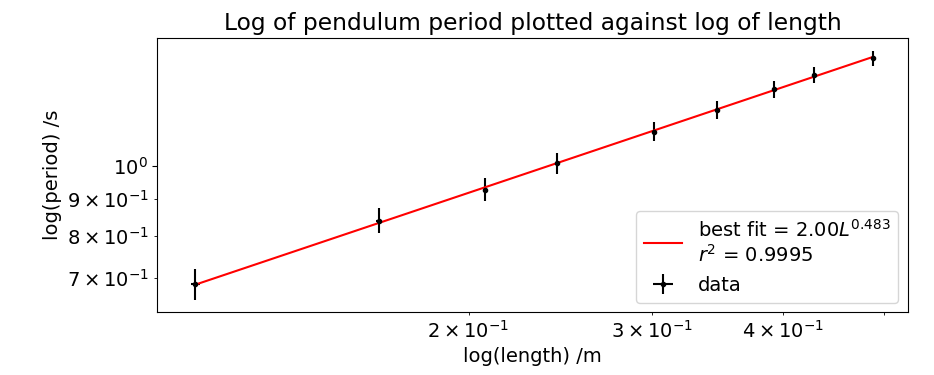
\includegraphics[width=\linewidth]{../figures/period_vs_length_log.png}
    \caption[]{Figure \ref{fig:figure 6} plotted with a log-log graph}
    \label{fig:figure 7}
\end{figure}

Taking log on both sides of Equation \ref{eq:l-over-g} turns it into the form of $y = mx + b$ where the slope of the line $m$ equals to the power $n$. Plotting on a logarithmic axis provides a useful way to analyze functions that obey a power law, revealing a linear graph as demonstrated by Figure \ref{fig:figure 7}. This reinforces the idea that Equation \ref{eq:l-over-g} is an accurate way of modelling the relationship between pendulum period and length.


\section{Q Factor and Length}

\subsection{Experimental Setup}
The same setup from Subsection \ref{sec 4.1 experimental setup} and the same lengths from Subsection \ref{sec 5.1 experimental setup} were used to collect data for Q factor calculation.

\subsection{Data}
The Q factor for every length was calculated by using Equation \ref{eq:q-factor-formula} with generated values of $\tau$ and $T$ as demonstrated in Subsection \ref{sec 4.3 analysis} because the uncertainty is smaller in general. The Q factor plot for all 9 lengths is shown below:

\begin{figure}[H]
    \centering
    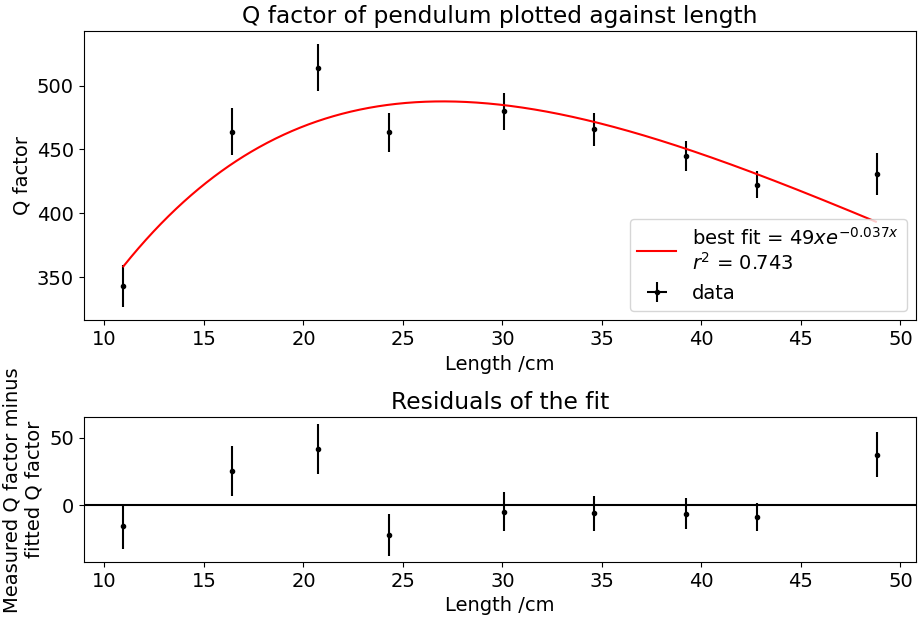
\includegraphics[width=\linewidth]{../figures/qfactor_vs_length.png}
    \caption{\centering Graph of Q factor plotted against pendulum length}
    \label{fig:figure 8}
\end{figure}

Calculations for each length and their uncertainties were outlined in Subsection \ref{sec 5.2 data}. The Q factors and their uncertainties were calculated by using Equation \ref{eq:q-factor-formula} since it was determined to be more optimal than the counting method.

\subsection{Analysis} \label{sec 6.3 analysis}
Unlike previous graphs, the Q factor plot seems to be a lot more erratic. This results in a best-fit line that does not fit nearly as perfect, suggested by the somewhat low $r^2$ value, and residuals that are both large and inconsistent. However a general increasing-decreasing trend can be identified, with the Q factor peaking at a certain value. Starting with a pendulum length of 10\,cm, the Q factor increases until a maximum in between lengths of 25\,cm-30\,cm then decreases as length increases to 50\,cm. This phenomenon could be explained with Equation \ref{eq:propto v} and Equation \ref{eq:propto v2} as follows.

At any length, $F_p$ and $F_d$ are always acting on the pendulum. However, the way in which they increase differs as length increase. If $F_p = c_1v$ and $F_d = c_2Av^2$, these two curves are guaranteed to intersect for some pendulum length. Therefore, towards the left of the intersection point is where $F_p$ dominates ($F_p > F_d$), indicated by the increasing behaviour and towards the right $F_d$ dominates ($F_p < F_d$), indicated by the decreasing behaviour.
A longer string released at the same angle in comparison to a shorter string will store more gravitational potential energy to be converted to kinetic energy, implying higher tangential velocity. Additionally, a longer string also increases the total surface area subjected to drag.

Modelling the Q factor graph in terms of an exponential, quadratic, sinusoidal, or power law function makes zero sense because intuitively, the Q factor should be 0 when the string length equals 0, and the Q factor should approach 0 when the string length approaches infinity. A function that seems to satisfy these constraints, used as the curve of best-fit for Figure \ref{fig:figure 8} is given by:
\begin{equation} \label{eq:crit-damp}
    Axe^{-bx}
\end{equation}
for $x \geq 0$ where:
{
\setlength{\abovedisplayskip}{2.5pt}
\begin{flalign*}
    \qquad A &= 49 \pm 3 & \\ % \\[-3pt] for paragraphs
    % \qqquad &\phantom{{}={}} \text{ayo continuation br}\\
    \qquad b &= 0.037 \pm 0.001 &
\end{flalign*}
}

\noindent which comes from the general shape of a critically damped oscillating system \cite{crit-damping}.

Due to the use of intuition, it cannot be concluded that Equation \ref{eq:crit-damp} is the correct relationship between Q factor and length, but it serves as a decent model in explaining how Q factor definitely depends on pendulum length.

\section{Conclusion}
In summary, Subsection \ref{sec 3.3 analysis} demonstrated that period is related to release angle and is symmetric for positive and negative release angles. Subsection \ref{sec 4.3 analysis} showed that for small angles, the damped harmonic oscillator model provides a good exponential fit for amplitude vs. time data. This can be used to find the Q factor with Equation \ref{eq:q-factor-formula} or counting, the former preferred since it carries a lower uncertainty. Subsection \ref{sec 5.3 analysis} presented a square root relationship between period and length, which was confirmed with a log-log plot. Finally, Subsection \ref{sec 6.3 analysis} shows that Q factor reaches a maximum of 487 when $L = 27\,\text{cm}$. The erratic measurements of Q factor resulted in a mediocre best-fit equation that was chosen based off intuition.

The largest uncertainty undoubtedly comes from measuring the maximum angles for amplitude due to the effect of camera skew on a double stringed contraption. This would result in many possible fits that pass through all error bars in the amplitude-time graph, propagating this error into the $\tau$ value used to calculate the Q factor. To reduce this error, digital measurement tools that exceed the budget of a homemade pendulum may be used to accurately track the pendulum's center of mass.

\newpage

\end{multicols}

\printbibliography[heading=bibintoc]

\newpage

\appendix

% \subfile{appendix.tex}

\end{document}
